%===============================================================
% Hashmon — Academic Technical Presentation
% Theme: Metropolis (refined academic style)
% Compile: pdfLaTeX or XeLaTeX on Overleaf
% Images: All placed in Overleaf project root
%===============================================================

\documentclass[aspectratio=169, 10pt]{beamer}

%---------------------------------------------------------------
% Theme & Packages
%---------------------------------------------------------------
\usetheme[progressbar=frametitle, numbering=fraction, sectionpage=progressbar]{metropolis}
\usepackage{appendixnumberbeamer}
\usepackage{amsmath}
\usepackage{array}
\usepackage{booktabs}
\usepackage{graphicx}
\usepackage{hyperref}
\usepackage{tikz}
\usepackage{xcolor}
\usetikzlibrary{arrows.meta, positioning, shapes.geometric, calc, fit}

%---------------------------------------------------------------
% Academic Colour Palette (colorblind-safe, WCAG AA)
%---------------------------------------------------------------
\definecolor{positive}{HTML}{0173B2}
\definecolor{negative}{HTML}{DE8F05}
\definecolor{emphasis}{HTML}{029E73}
\definecolor{neutral}{gray}{0.55}
\definecolor{layerA}{HTML}{DAEAF6}   % blue tint
\definecolor{layerB}{HTML}{FDE8D0}   % orange tint
\definecolor{layerC}{HTML}{D4EFDF}   % green tint
\definecolor{layerD}{HTML}{E8DAEF}   % purple tint

\newcommand{\pos}[1]{\textcolor{positive}{#1}}
\newcommand{\con}[1]{\textcolor{negative}{#1}}
\newcommand{\HL}[1]{\textcolor{emphasis}{#1}}

%---------------------------------------------------------------
% Beamer Refinements
%---------------------------------------------------------------
\setbeamertemplate{navigation symbols}{}
\setbeamerfont{footnote}{size=\tiny}
\setbeamercolor{progress bar}{fg=positive, bg=positive!15}
\metroset{block=fill}

%---------------------------------------------------------------
% Reusable TikZ Styles
%---------------------------------------------------------------
\tikzset{
  layer/.style={
    rounded corners=3pt, fill=#1, draw=gray,
    minimum width=11cm, minimum height=1.2cm,
    font=\small, align=center, thick, text width=10.5cm,
    inner sep=5pt
  },
  layer/.default=layerA,
  flowbox/.style={
    draw=gray!70, rounded corners=5pt, fill=positive!6,
    minimum width=2.1cm, minimum height=0.95cm,
    font=\small, align=center, thick
  },
  darrow/.style={-{Latex[length=2mm, width=1.6mm]}, semithick, color=neutral},
  biarrow/.style={{Latex[length=2mm, width=1.6mm]}-{Latex[length=2mm, width=1.6mm]}, semithick, color=neutral}
}

%---------------------------------------------------------------
% Title Page
%---------------------------------------------------------------
\title{Hashmon}
\subtitle{A User-Generated, Cross-Game Digital Companion Ecosystem}
\author{Baohua Fang\\{\small Student ID: 123090108}}
\date{FTE4312 --- Spring 2026}
\institute{School of Science and Engineering}
\titlegraphic{\hfill
\includegraphics[width=0.24\linewidth,keepaspectratio]{HashmonLogo.jpg}}

%===============================================================
\begin{document}
%===============================================================

\maketitle

%---------------------------------------------------------------
% Outline
%---------------------------------------------------------------
\begin{frame}{Outline}
  \tableofcontents
\end{frame}

%===============================================================
\section{Motivation \& Problem}
%===============================================================

%---------------------------------------------------------------
% Personal Motivation
%---------------------------------------------------------------
\begin{frame}{Personal Motivation}
  \begin{columns}[T]
    \begin{column}{0.42\textwidth}
      \centering
      
\includegraphics[width=\linewidth,height=5.2cm,keepaspectratio]{eevee.jpg}
    \end{column}
    \begin{column}{0.50\textwidth}
      \begin{alertblock}{A personal story}
        I raised an Eevee that felt like a real companion ---
        but its existence ended when the game did.
      \end{alertblock}
      \vspace{0.3cm}
      \begin{itemize}
        \item Emotional bond formed through gameplay
        \item No way to export or reuse the companion
        \item \HL{That regret inspired Hashmon}
      \end{itemize}
    \end{column}
  \end{columns}
\end{frame}

%---------------------------------------------------------------
% The Problem
%---------------------------------------------------------------
\begin{frame}{The Problem: Companions Are Platform-Locked}
  \begin{columns}[T]
    \begin{column}{0.40\textwidth}
      \centering
      
\includegraphics[width=\linewidth,height=5.0cm,keepaspectratio]{Pokemon.jpg}
    \end{column}
    \begin{column}{0.55\textwidth}
      \textbf{Players invest:} time, emotion, creativity
      \vspace{0.3cm}

      \textbf{Current games provide:}
      \begin{itemize}
        \item \con{Closed ownership} --- assets locked to one platform
        \item \con{No portability} --- cannot move across games
        \item \con{No persistence} --- progress lost at shutdown
      \end{itemize}
      \vspace{0.3cm}
      \begin{block}{Gap}
        No lightweight framework lets players \emph{own} and
        \emph{reuse} companions across game contexts.
      \end{block}
    \end{column}
  \end{columns}
\end{frame}

%---------------------------------------------------------------
% Research Question & Contributions
%---------------------------------------------------------------
\begin{frame}{Research Question \& Contributions}
  \begin{alertblock}{Research Question}
    Can a single NFT-based companion maintain meaningful identity
    and utility across multiple independent game scenes?
  \end{alertblock}
  \vspace{0.4cm}
  \textbf{Contributions:}
  \begin{enumerate}
    \item \pos{End-to-end prototype} integrating browser gameplay
          with on-chain ownership (ERC-721)
    \item \pos{Cross-scene reuse} --- one NFT drives battle,
          garden, and marketplace contexts
    \item \pos{Decentralised asset pipeline} via IPFS for
          metadata and artwork storage
    \item \pos{In-game marketplace} enabling peer-to-peer
          companion trading on Sepolia testnet
  \end{enumerate}
\end{frame}

%===============================================================
\section{System Design}
%===============================================================

%---------------------------------------------------------------
% System Architecture
%---------------------------------------------------------------
\begin{frame}{System Architecture}
  \vspace{0.05cm}
  %--- Logo row ---
  \begin{columns}[T]
    \begin{column}{0.24\textwidth}
      \centering
      
\includegraphics[width=0.60\linewidth,height=0.80cm,keepaspectratio]{HashmonLogo.jpg}\\[0.04cm]
      
\includegraphics[width=0.60\linewidth,height=0.70cm,keepaspectratio]{PhaserLogo.png}\\[0.08cm]
      {\footnotesize\textbf{Game Client}}
    \end{column}
    \begin{column}{0.24\textwidth}
      \centering
      
\includegraphics[width=0.60\linewidth,height=0.70cm,keepaspectratio]{MetaMaskLogo.png}\\[0.04cm]
      
\includegraphics[width=0.60\linewidth,height=0.50cm,keepaspectratio]{etherjs.jpg}\\[0.08cm]
      {\footnotesize\textbf{Wallet Layer}}
    \end{column}
    \begin{column}{0.24\textwidth}
      \centering
      
\includegraphics[width=0.60\linewidth,height=0.70cm,keepaspectratio]{SepoilaLogo.png}\\[0.52cm]
      {\footnotesize\textbf{Blockchain}}
    \end{column}
    \begin{column}{0.24\textwidth}
      \centering
      \fbox{\parbox[c][0.70cm][c]{0.60\linewidth}{\centering\textbf{IPFS}}}\\[0.52cm]
      {\footnotesize\textbf{Storage Layer}}
    \end{column}
  \end{columns}

  \vspace{0.15cm}
  %--- Layered architecture diagram ---
  \centering
  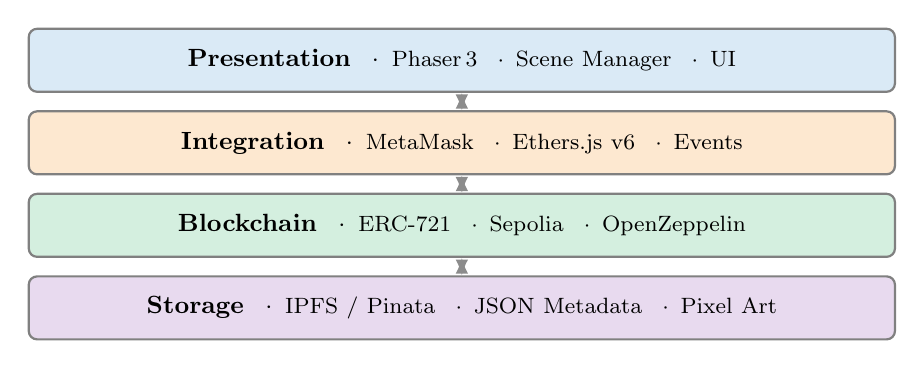
\begin{tikzpicture}[node distance=0.22cm]
    \node[layer=layerA, minimum height=0.80cm] (L4) {%
      \textbf{Presentation} \enspace$\cdot$\enspace
      {\footnotesize Phaser\,3 \enspace$\cdot$\enspace
       Scene Manager \enspace$\cdot$\enspace UI}};

    \node[layer=layerB, minimum height=0.80cm, below=of L4] (L3) {%
      \textbf{Integration} \enspace$\cdot$\enspace
      {\footnotesize MetaMask \enspace$\cdot$\enspace
       Ethers.js v6 \enspace$\cdot$\enspace Events}};

    \node[layer=layerC, minimum height=0.80cm, below=of L3] (L2) {%
      \textbf{Blockchain} \enspace$\cdot$\enspace
      {\footnotesize ERC-721 \enspace$\cdot$\enspace
       Sepolia \enspace$\cdot$\enspace OpenZeppelin}};

    \node[layer=layerD, minimum height=0.80cm, below=of L2] (L1) {%
      \textbf{Storage} \enspace$\cdot$\enspace
      {\footnotesize IPFS / Pinata \enspace$\cdot$\enspace
       JSON Metadata \enspace$\cdot$\enspace Pixel Art}};

    \draw[biarrow] (L4) -- (L3);
    \draw[biarrow] (L3) -- (L2);
    \draw[biarrow] (L2) -- (L1);
  \end{tikzpicture}
\end{frame}

%---------------------------------------------------------------
% Workflow
%---------------------------------------------------------------
\begin{frame}{Workflow: From Creation to Reuse}
  \centering
  \vspace{0.15cm}
  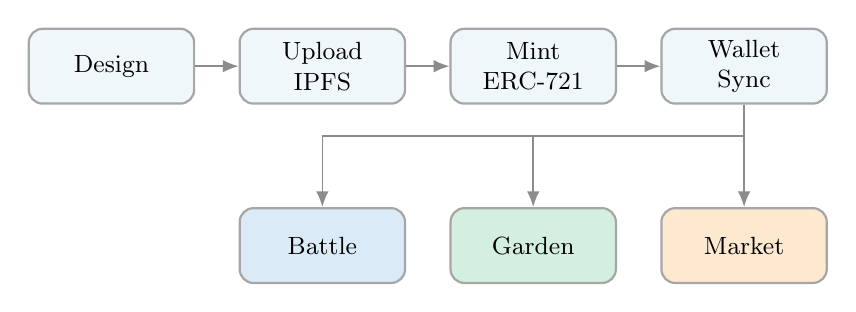
\begin{tikzpicture}[node distance=0.55cm, every node/.style={font=\small, align=center}]
    % Pipeline
    \node[flowbox] (c) {Design};
    \node[flowbox, right=of c] (u) {Upload\\IPFS};
    \node[flowbox, right=of u] (m) {Mint\\ERC-721};
    \node[flowbox, right=of m] (s) {Wallet\\Sync};

    % Scene targets
    \node[flowbox, fill=layerA, below=1.3cm of u] (b) {Battle};
    \node[flowbox, fill=layerC, below=1.3cm of m] (g) {Garden};
    \node[flowbox, fill=layerB, below=1.3cm of s] (mk) {Market};

    % Pipeline arrows
    \draw[darrow] (c) -- (u);
    \draw[darrow] (u) -- (m);
    \draw[darrow] (m) -- (s);

    % Fan-out from Sync to scenes
    \path (s.south) ++(0,-0.4) coordinate (fork);
    \draw[thick, color=neutral] (s.south) -- (fork);
    \draw[thick, color=neutral] (fork) -- (fork -| b.north);
    \draw[darrow] (fork -| b.north) -- (b.north);
    \draw[darrow] (fork -| g.north) -- (g.north);
    \draw[darrow] (fork) -- (mk.north);
  \end{tikzpicture}

  \vspace{0.35cm}
  \begin{block}{Key Property}
    A single NFT companion is created once, owned cryptographically,
    and reused across all game scenes.
  \end{block}
\end{frame}

%===============================================================
\section{Prototype Evidence}
%===============================================================

%---------------------------------------------------------------
% Create & Mint
%---------------------------------------------------------------
\begin{frame}{Evidence: Create \& Mint}
  \begin{columns}[T]
    \begin{column}{0.48\textwidth}
      \centering
      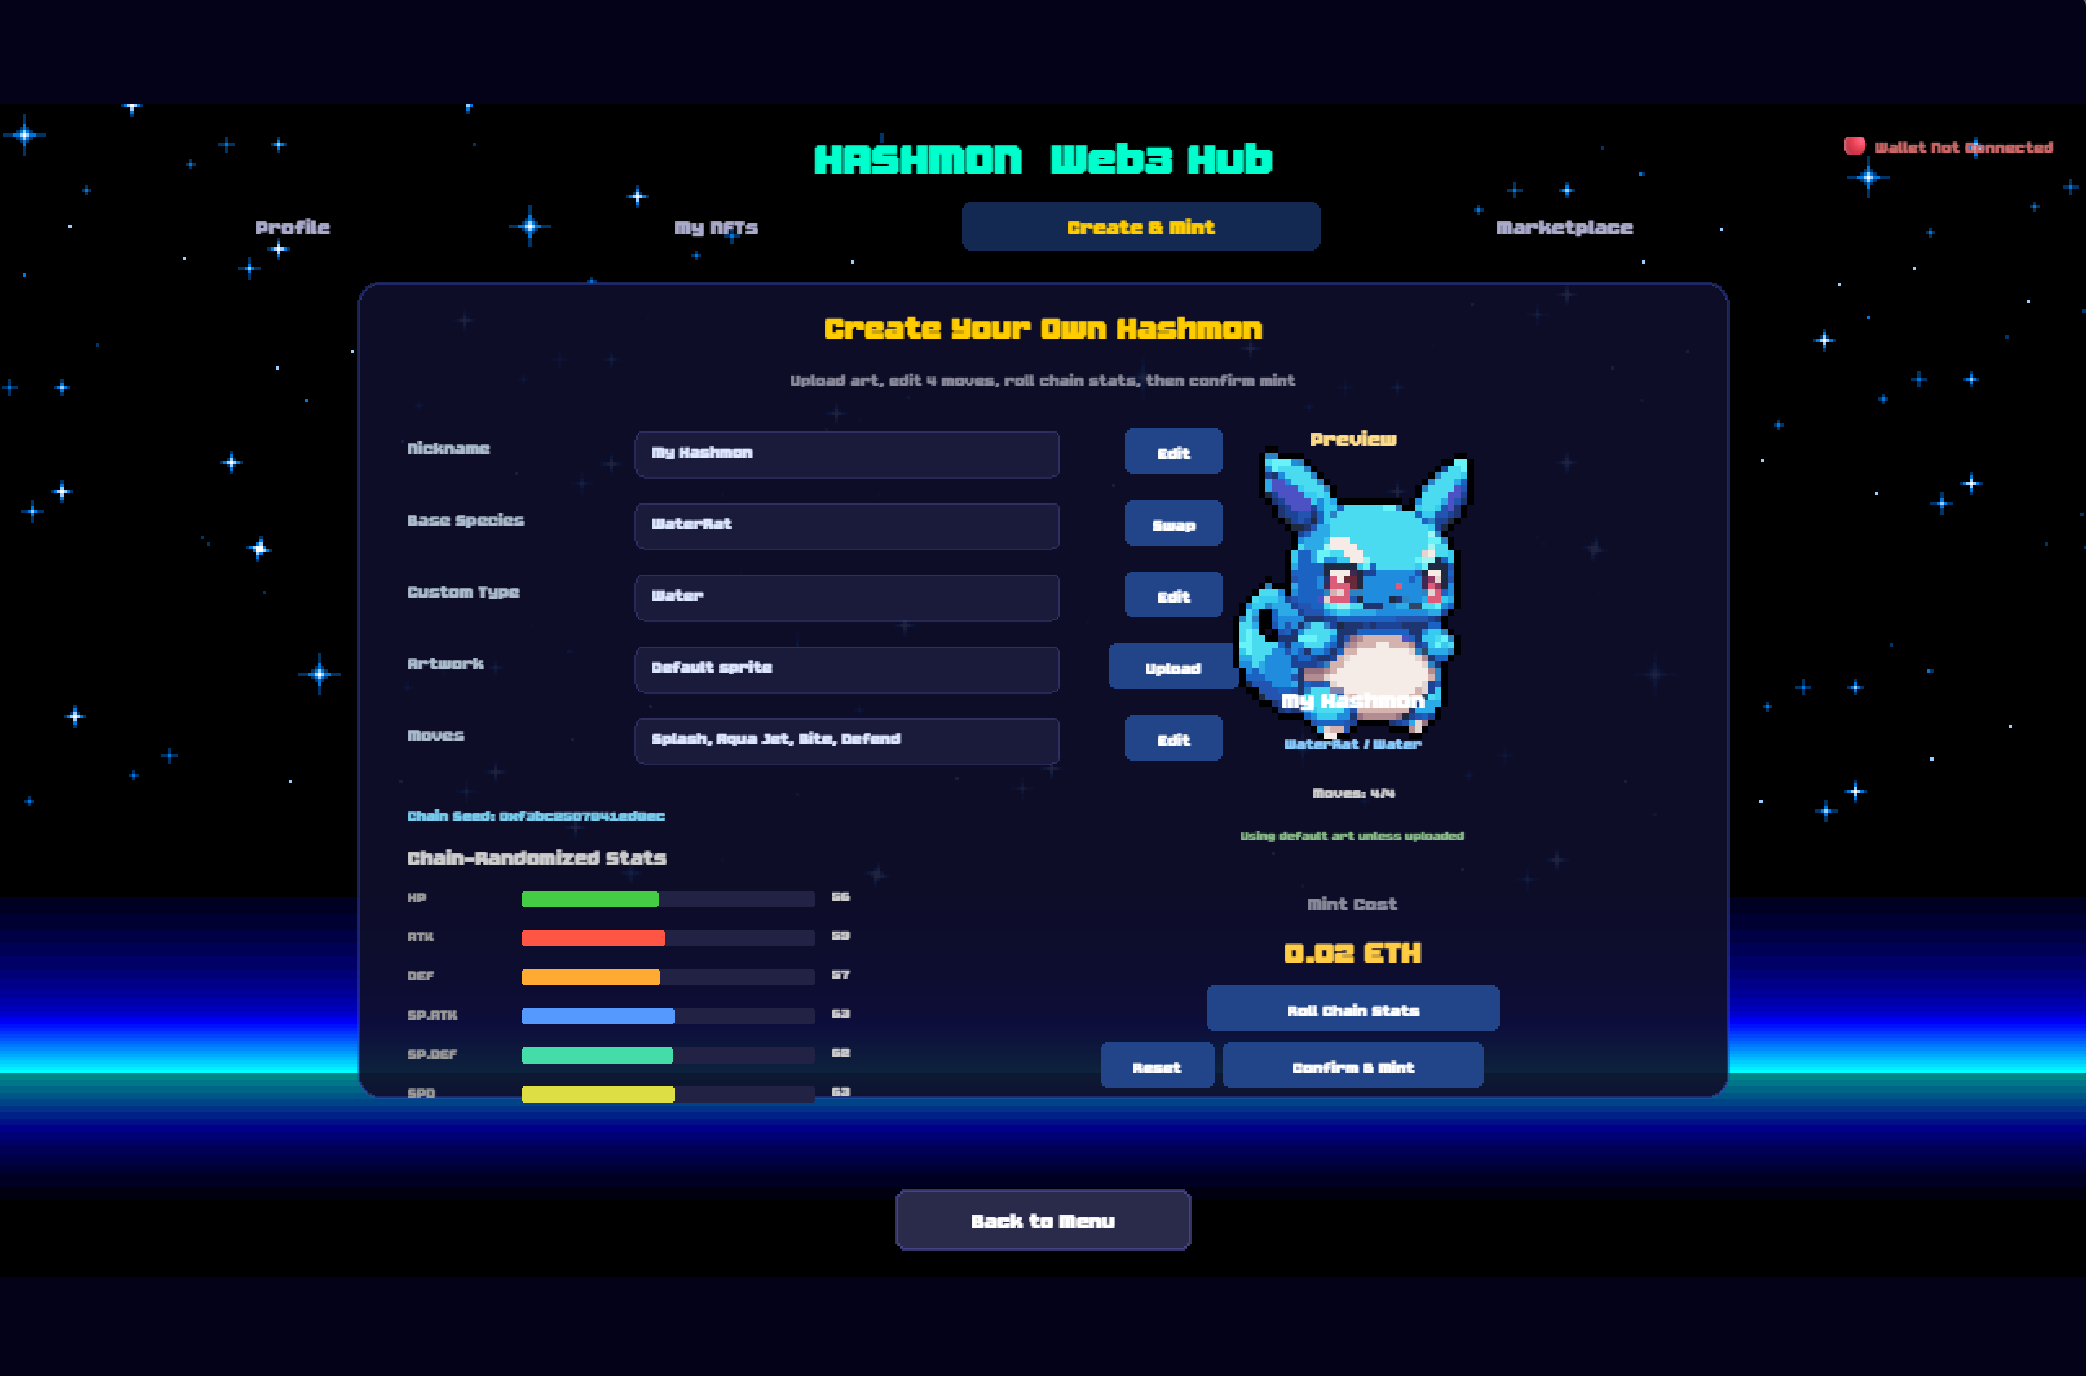
\includegraphics[width=\linewidth,height=4.8cm,keepaspectratio]{CreateMint.png}\\[0.12cm]
      {\footnotesize\color{neutral}(a) Custom companion designer}
    \end{column}
    \begin{column}{0.48\textwidth}
      \centering
      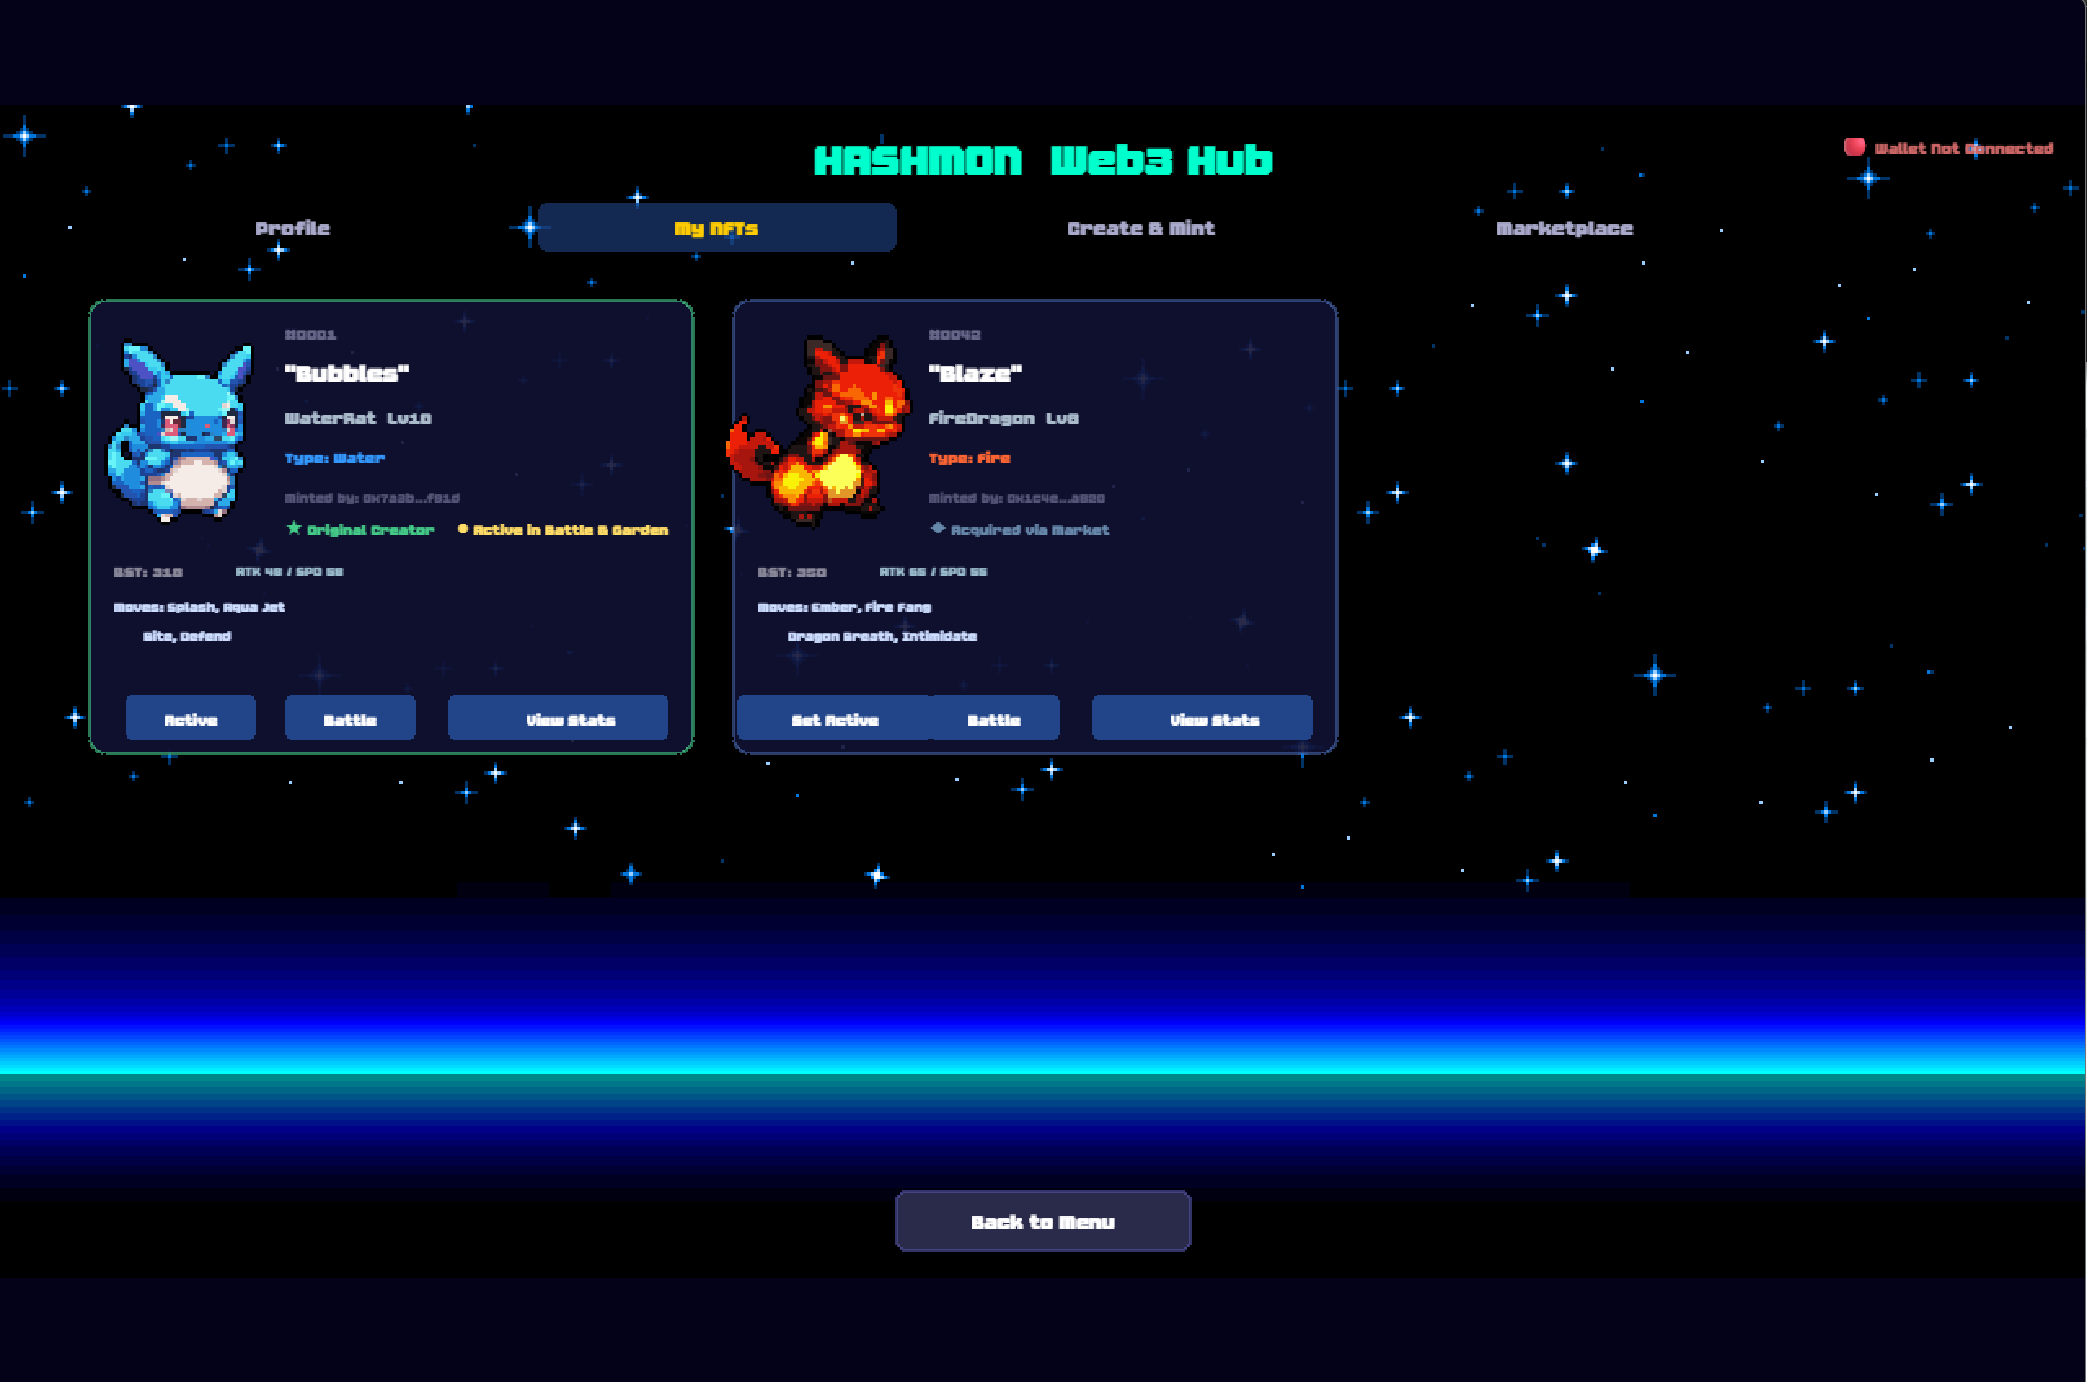
\includegraphics[width=\linewidth,height=4.8cm,keepaspectratio]{MyNFTs.png}\\[0.12cm]
      {\footnotesize\color{neutral}(b) Wallet-synced NFT inventory}
    \end{column}
  \end{columns}
  \vspace{0.25cm}
  \begin{itemize}
    \item Player designs pixel-art companion, mints as ERC-721
    \item Inventory reflects on-chain ownership in real time
  \end{itemize}
\end{frame}

%---------------------------------------------------------------
% Cross-Scene Interoperability
%---------------------------------------------------------------
\begin{frame}{Evidence: Cross-Scene Interoperability}
  \begin{columns}[T]
    \begin{column}{0.48\textwidth}
      \centering
      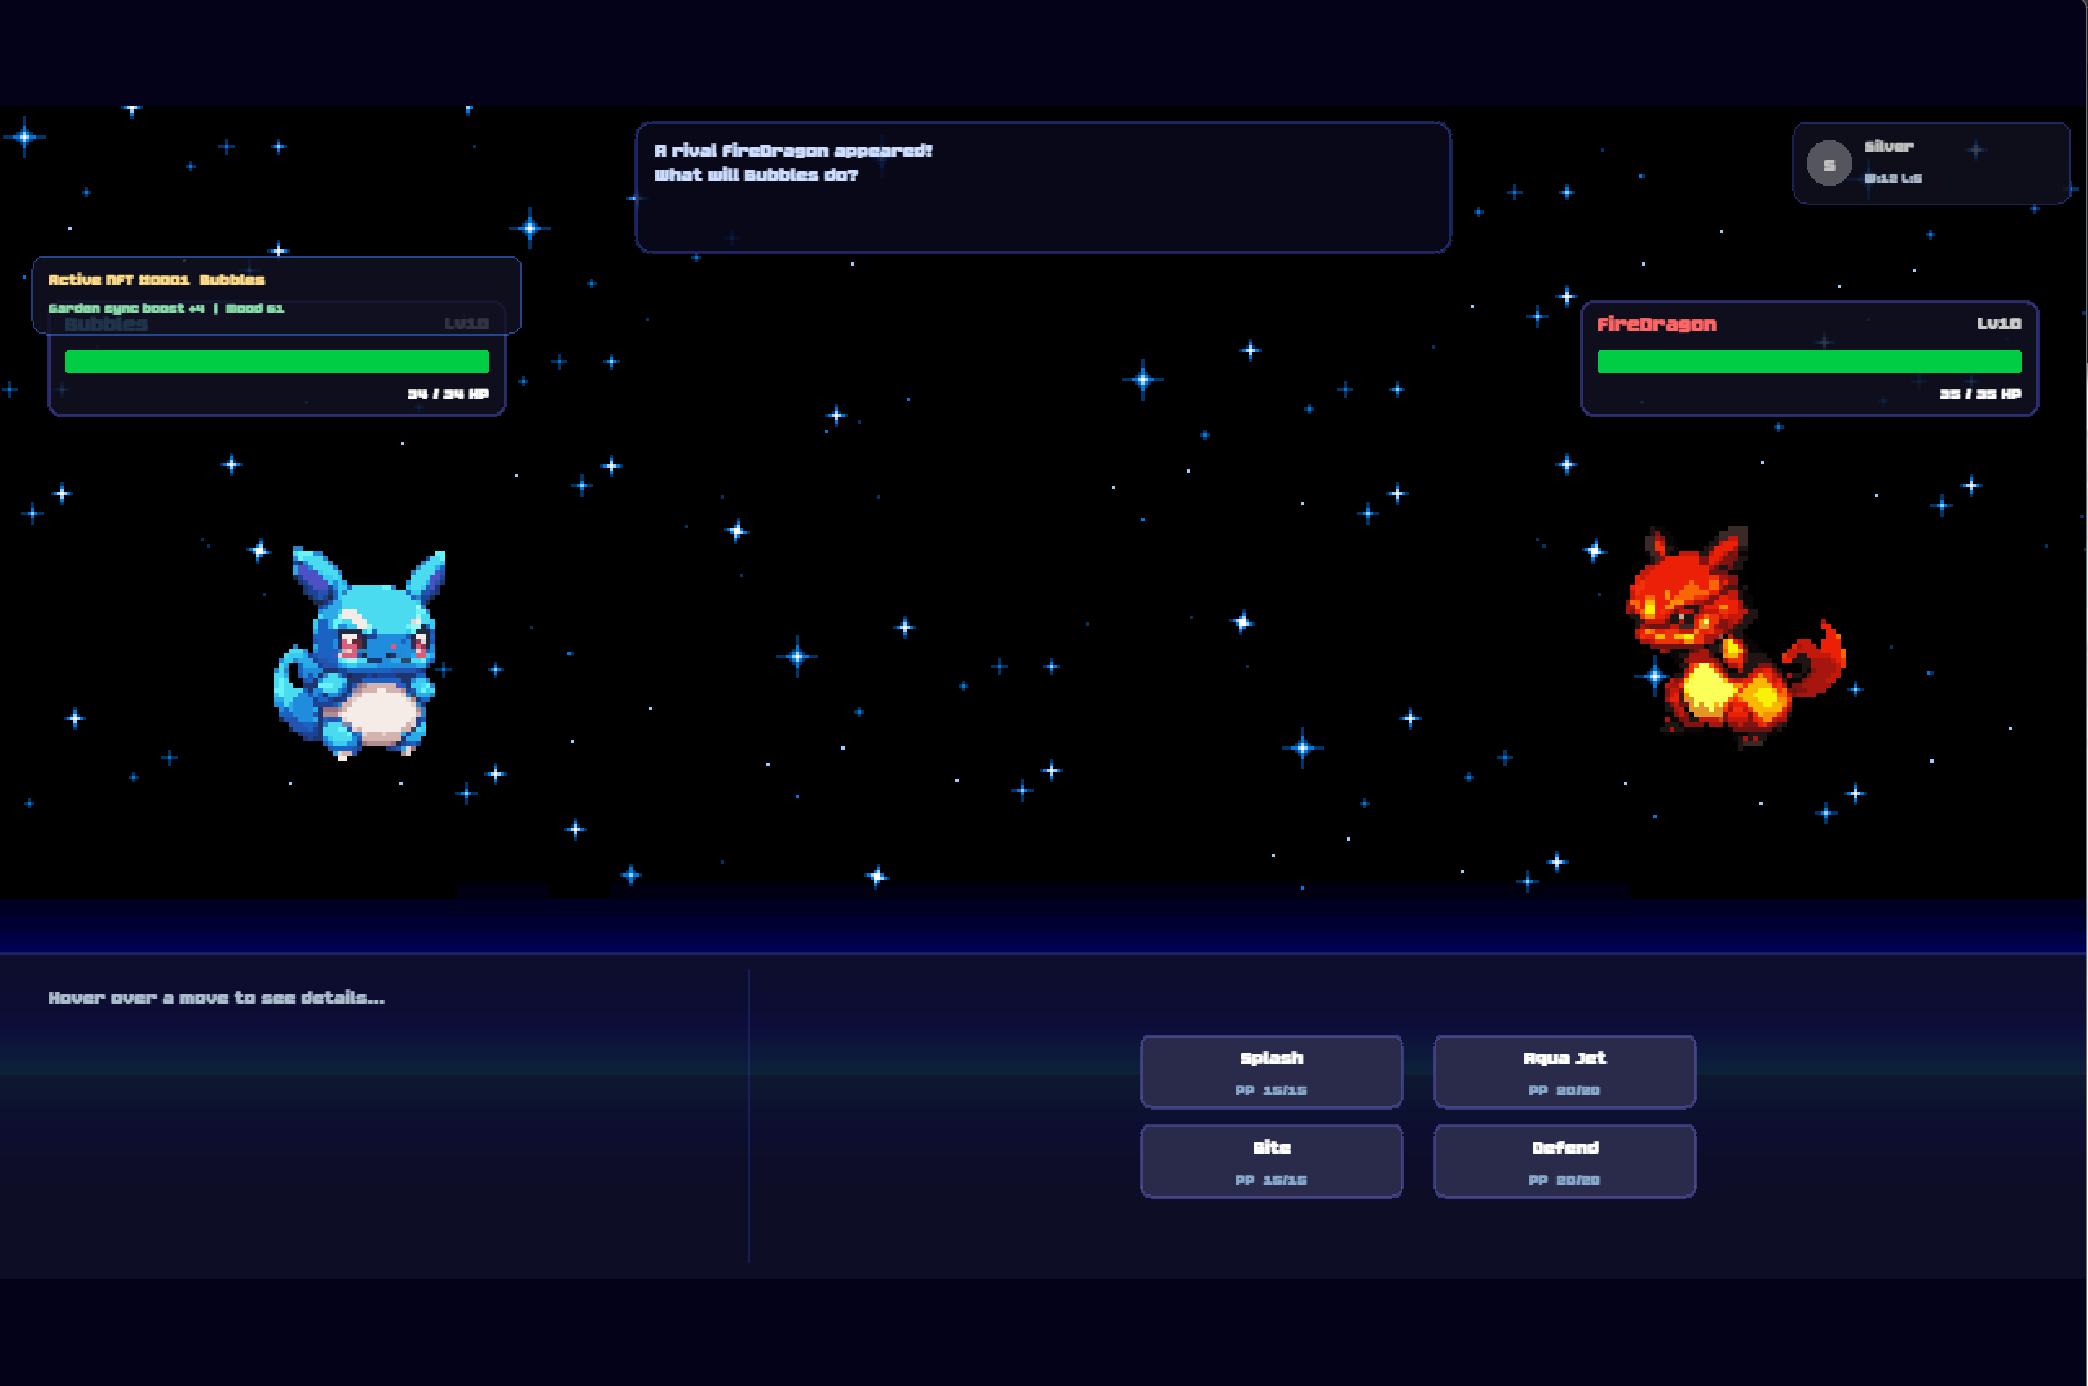
\includegraphics[width=\linewidth,height=4.0cm,keepaspectratio]{BattleScene.png}\\[0.1cm]
      {\footnotesize\color{neutral}(a) Battle --- stats-driven combat}
    \end{column}
    \begin{column}{0.48\textwidth}
      \centering
      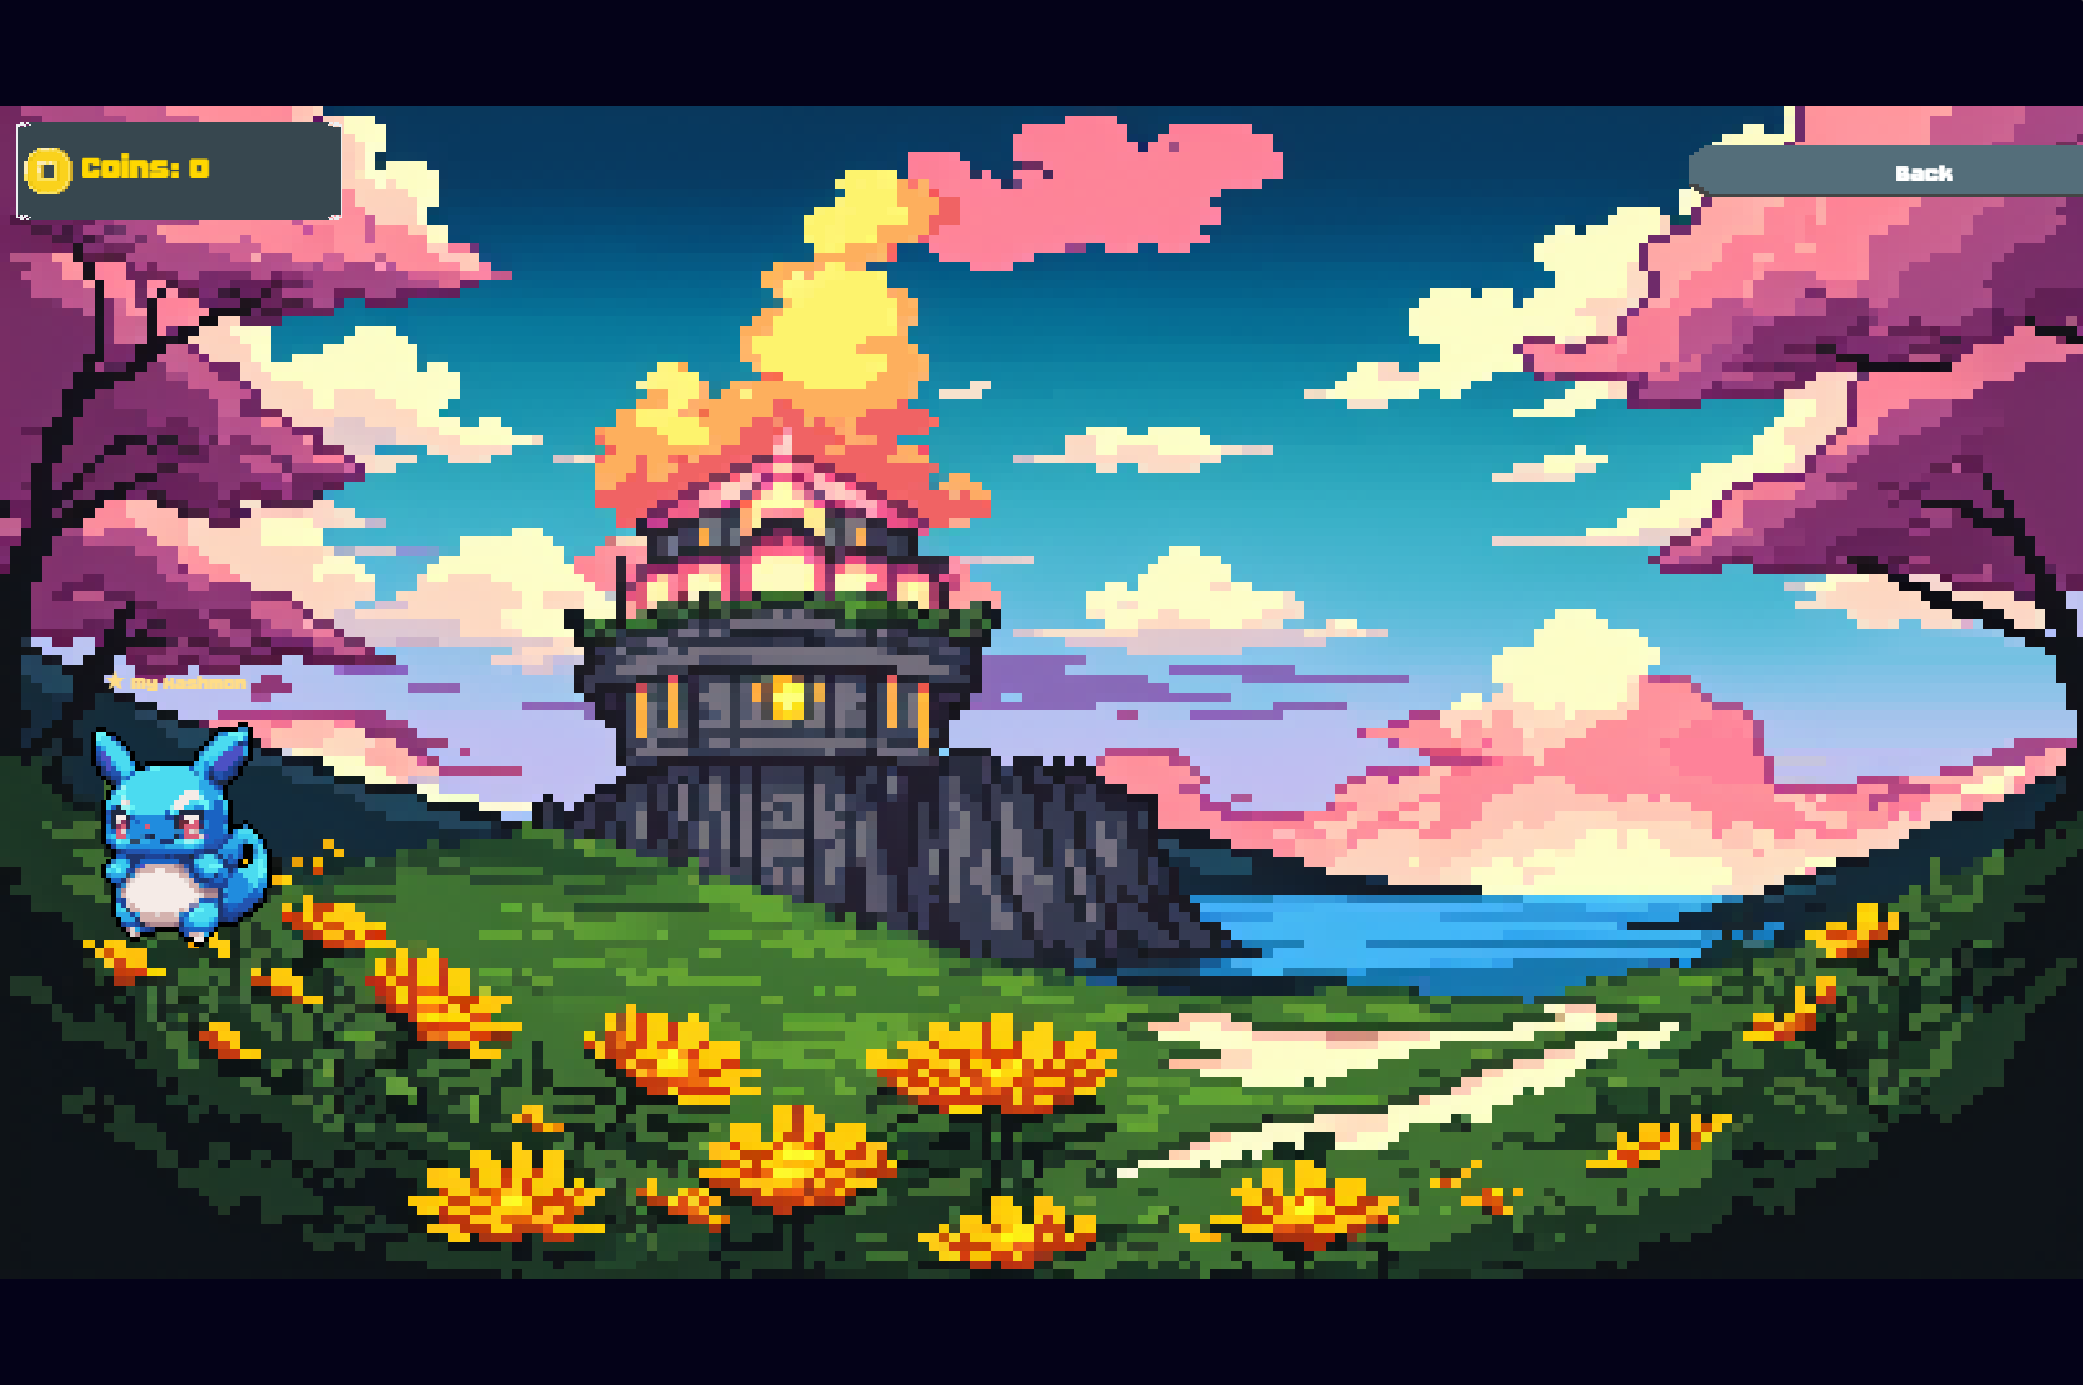
\includegraphics[width=\linewidth,height=4.0cm,keepaspectratio]{GardenScene.png}\\[0.1cm]
      {\footnotesize\color{neutral}(b) Garden --- mood and movement}
    \end{column}
  \end{columns}
  \vspace{0.25cm}
  \begin{block}{Observation}
    The \emph{same} NFT drives behaviour in structurally different
    game contexts, demonstrating controlled interoperability.
  \end{block}
\end{frame}

%---------------------------------------------------------------
% Marketplace
%---------------------------------------------------------------
\begin{frame}{Evidence: Marketplace \& Ownership Loop}
  \begin{columns}[T]
    \begin{column}{0.55\textwidth}
      \centering
      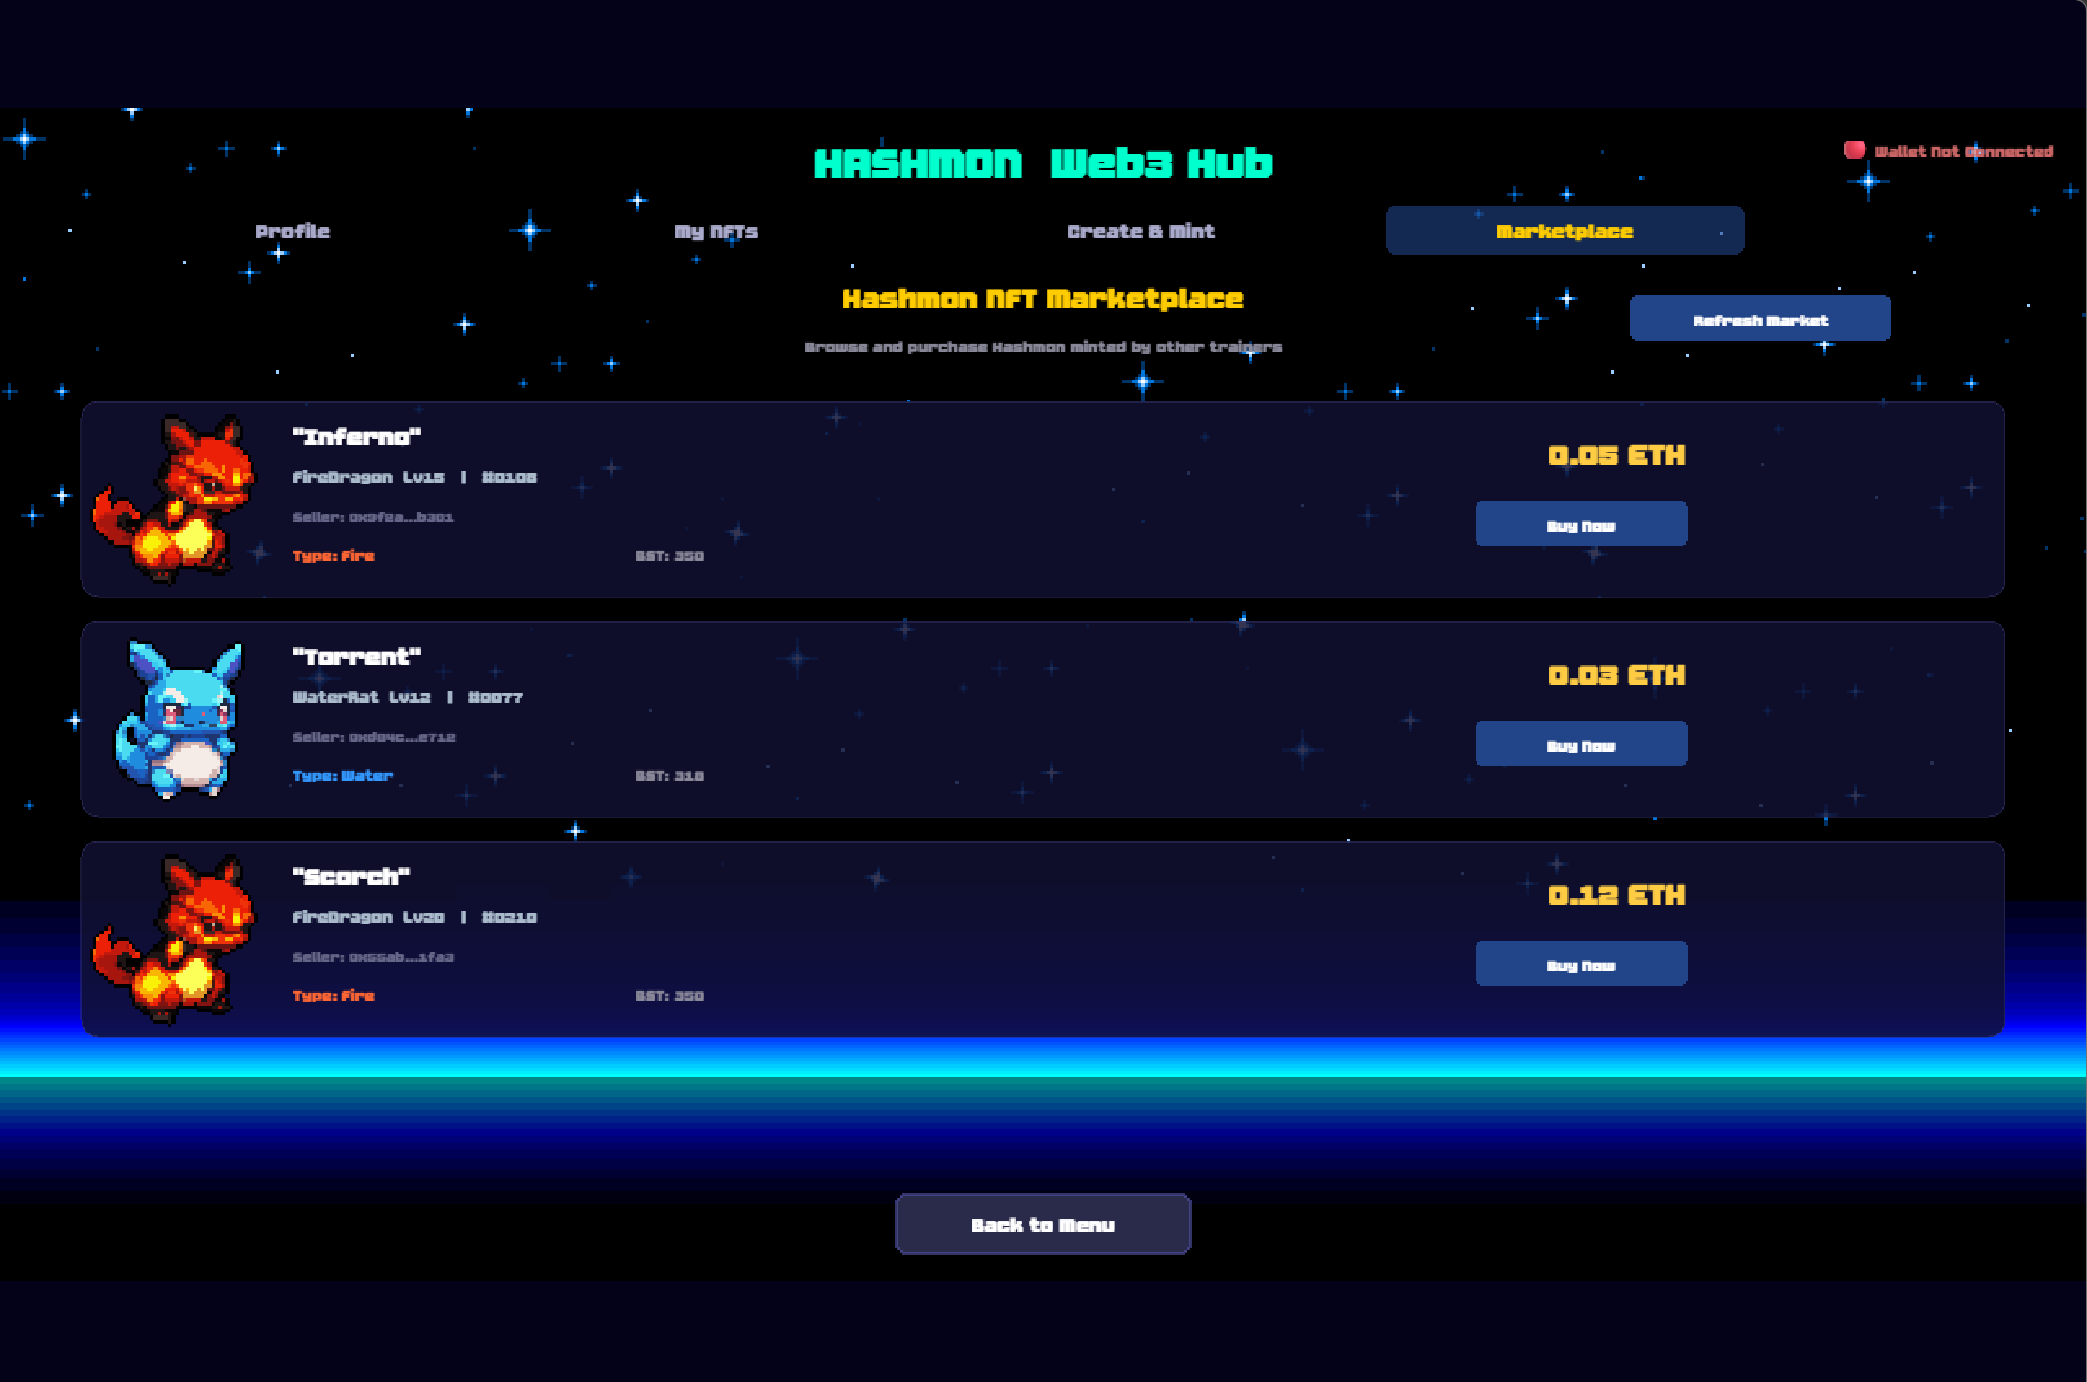
\includegraphics[width=\linewidth,height=4.8cm,keepaspectratio]{MarketPlace.png}\\[0.1cm]
      {\footnotesize\color{neutral}Peer-to-peer marketplace on Sepolia}
    \end{column}
    \begin{column}{0.40\textwidth}
      \vspace{0.2cm}
      \textbf{Functionality:}
      \begin{itemize}
        \item List companions for sale
        \item Browse all listed assets
        \item Purchase via MetaMask
        \item On-chain ownership transfer
      \end{itemize}
      \vspace{0.15cm}
      \begin{exampleblock}{Implication}
        Companions gain economic value
        beyond gameplay utility.
      \end{exampleblock}
    \end{column}
  \end{columns}
\end{frame}

%===============================================================
\section{Evaluation \& Conclusion}
%===============================================================

%---------------------------------------------------------------
% Results & Limitations
%---------------------------------------------------------------
\begin{frame}{Results \& Current Limitations}
  \centering
  \vspace{0.1cm}
  \begin{tabular}{
    >{\raggedright}p{0.40\linewidth}
    >{\raggedright\arraybackslash}p{0.40\linewidth}}
    \toprule
    \textbf{\pos{Prototype Demonstrates}} & \textbf{\con{Open Challenges}} \\
    \midrule
    Wallet-based authentication    & Multi-chain support \\
    On-chain NFT minting (ERC-721) & Deeper gameplay mechanics \\
    IPFS-hosted metadata \& art    & Cross-project standard adoption \\
    Cross-scene companion reuse    & Game balance across contexts \\
    Peer-to-peer marketplace       & UI polish \& user testing \\
    \bottomrule
  \end{tabular}
  \vspace{0.3cm}
  \begin{block}{Summary}
    Five core Web3 interactions verified end-to-end on Sepolia;
    limitations are engineering scope, not architectural.
  \end{block}
\end{frame}

%---------------------------------------------------------------
% Future Work
%---------------------------------------------------------------
\begin{frame}{Future Work}
  \centering
  \vspace{0.15cm}
  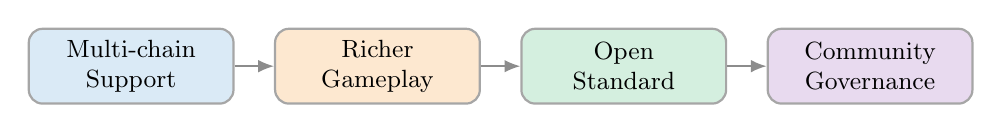
\begin{tikzpicture}[node distance=0.5cm, every node/.style={font=\small, align=center}]
    \node[flowbox, fill=layerA, minimum width=2.6cm] (s1) {Multi-chain\\Support};
    \node[flowbox, fill=layerB, minimum width=2.6cm, right=of s1] (s2) {Richer\\Gameplay};
    \node[flowbox, fill=layerC, minimum width=2.6cm, right=of s2] (s3) {Open\\Standard};
    \node[flowbox, fill=layerD, minimum width=2.6cm, right=of s3] (s4) {Community\\Governance};

    \draw[darrow] (s1) -- (s2);
    \draw[darrow] (s2) -- (s3);
    \draw[darrow] (s3) -- (s4);
  \end{tikzpicture}

  \vspace{0.4cm}
  \begin{itemize}
    \item Extend to Polygon / Arbitrum for lower transaction costs
    \item Integrate evolution mechanics and breeding systems
    \item Propose open companion metadata standard (EIP draft)
    \item Transition marketplace governance to DAO structure
  \end{itemize}
\end{frame}

%---------------------------------------------------------------
% References (second-to-last, before Thank You)
%---------------------------------------------------------------
\begin{frame}{References}
  \small
  \begin{thebibliography}{6}
    \bibitem{erc721}
      W.\,Entriken et al.,
      ``ERC-721: Non-Fungible Token Standard,''
      Ethereum EIP, 2018.
    \bibitem{ipfs}
      J.\,Benet,
      ``IPFS --- Content Addressed, Versioned, P2P File System,''
      \textit{arXiv:1407.3561}, 2014.
    \bibitem{oz}
      OpenZeppelin,
      ``Contracts Documentation,'' 2026.
      \url{https://docs.openzeppelin.com/}
    \bibitem{ethers}
      Ethers.js,
      ``Documentation v6,'' 2026.
      \url{https://docs.ethers.org/}
    \bibitem{phaser}
      Phaser Studio,
      ``Phaser 3 Documentation,'' 2026.
      \url{https://docs.phaser.io/}
    \bibitem{metamask}
      MetaMask,
      ``Developer Documentation,'' 2026.
      \url{https://docs.metamask.io/}
  \end{thebibliography}
\end{frame}

%---------------------------------------------------------------
% Thank You
%---------------------------------------------------------------
\begin{frame}[standout]
  Hashmon\\[0.6em]
  \large A player-owned companion can survive\\
  across multiple gameplay contexts.\\[1.0em]
  \normalsize Thank you\\[0.3em]
  Questions welcome\\[0.8em]
  \small\color{gray}{\textit{A full end-to-end demo video will be played next.}}
\end{frame}

%===============================================================
\appendix
%===============================================================

%---------------------------------------------------------------
% Backup Slide 1: Cross-Game Detail
%---------------------------------------------------------------
\begin{frame}{Backup: Cross-Game Interoperability Detail}
  \centering
  \includegraphics[width=0.62\linewidth,height=5.5cm,keepaspectratio]%
    {StatusWithCrossGameInteroperabilityProof.png}\\[0.15cm]
  {\footnotesize\color{neutral}
   Same companion verified across Battle, Garden, and Inventory scenes.}
\end{frame}

%---------------------------------------------------------------
% Backup Slide 2: Technology Stack
%---------------------------------------------------------------
\begin{frame}{Backup: Technology Stack}
  \centering
  \vspace{0.15cm}
  \begin{tabular}{@{} l l l @{}}
    \toprule
    \textbf{Layer} & \textbf{Technology} & \textbf{Role} \\
    \midrule
    Frontend  & Phaser\,3 (JavaScript)   & Game engine \& scene management \\
    Wallet    & MetaMask + Ethers.js\,v6 & Transaction signing \& reads \\
    Contract  & Solidity + OpenZeppelin  & ERC-721 minting \& marketplace \\
    Network   & Sepolia Testnet          & Public Ethereum test environment \\
    Storage   & IPFS via Pinata          & Immutable metadata \& art hosting \\
    \bottomrule
  \end{tabular}
\end{frame}

%---------------------------------------------------------------
% Backup Slide 3: Smart Contract Interface
%---------------------------------------------------------------
\begin{frame}{Backup: Smart Contract Interface}
  \centering
  \vspace{0.1cm}
  \begin{tabular}{@{} l p{7.2cm} @{}}
    \toprule
    \textbf{Function} & \textbf{Description} \\
    \midrule
    \texttt{mintNFT(to, uri)}     & Mint new companion with IPFS metadata URI \\
    \texttt{tokenURI(id)}         & Retrieve metadata URI for a given token \\
    \texttt{listForSale(id, p)}   & List companion on marketplace at price \texttt{p} \\
    \texttt{buyNFT(id)}           & Purchase listed companion (payable) \\
    \texttt{ownerOf(id)}          & Query current owner address \\
    \bottomrule
  \end{tabular}
\end{frame}

\end{document}
